\documentclass{beamer}
\usetheme{metropolis} % Use metropolis theme


\title{ECON 3818: Introduction to Statistics with Computer Applications}
%\subtitle
\date{\today}
\author{Kyle Butts}

\definecolor{blue}{RGB}{0,114,178}
\definecolor{red}{HTML}{EB0E09}
\definecolor{yellow}{RGB}{240,228,66}
\definecolor{green}{RGB}{0,158,115}
\definecolor{maroon}{HTML}{AF3335}
\definecolor{purple}{HTML}{7E90B8}

\definecolor{mybackground}{HTML}{ECECEC}
\setbeamercolor{background canvas}{bg= mybackground}

\definecolor{buff-gold}{HTML}{CFB87C}
\definecolor{buff-grey}{HTML}{565A5C}
\definecolor{buff-lightgrey}{HTML}{A2A4A3}
\definecolor{buff-black}{HTML}{000000}

\setbeamercolor{alerted text}{fg=buff-gold!80!black}
\setbeamercolor{frametitle}{bg=buff-black}
\setbeamercolor{title}{fg=buff-grey}
\setbeamercolor{button}{bg=buff-gold}

% Allow to remove indent w/ \begin{itemize}[leftmargin= *]
\usepackage{enumitem}
\setlist[itemize]{label= \textbullet}

% \usepackage[libertine]{newtxmath}
\usepackage{longtable}
\usepackage{booktabs}
\usepackage{enumitem}

\begin{document}

% Title Page ---------------------------------------
\maketitle

% Estimation -------------------------------------
\section{Estimation}

\begin{itemize}
	\item We use the sample information to calculate sample statistics
	\item We are making inference about population parameters 
\end{itemize}
\vskip.4cm
To help us understand sample statistics we discussed two important theorems:
\begin{itemize}
	\item The Law of Large Numbers
	\item The Central Limit Theorem
\end{itemize}
\end{frame}

\begin{frame}{Clicker Question}
	Consider a simple random sample of size $n$, from a population with $\mu$ and a standard deviation $\sigma$. What does the Central Limit Theorem say about the sampling distribution of sample mean $\bar{X}$ when $n$ is large?
	\vskip.4cm
	\begin{enumerate}[label=(\alph*)]
		\item $\bar{X}$ has a mean $\mu$
		\item $\bar{X}$ is approximately normal
		\item $\bar{X}$ is only approximately normal if population distribution is normal
		\item $\bar{X}$ has the same shape as the population distribution
	\end{enumerate}
\end{frame}


\begin{frame}{Next Steps}
	To understand how well our sample statistic does in approximating the population parameters, we need to understand:
	\begin{itemize}
		\item The distribution of the sample statistic $\checkmark$
		\item How the sample statistic changes with sample size $\checkmark$
		\item How to rank sample statistics
	\end{itemize}
\end{frame}


\begin{frame}{Ranking Sample Statistics}
	Recall sample statistics are \textit{estimates}, or our best guesses, for population parameters
	\vskip.2cm
	We rank sample statistics based off their \alert{bias} and \alert{variance}
\end{frame}

\begin{frame}{Properties of Expectation and Variance}
	Reminder of the properties of expectation and variance:
	\begin{itemize}
		\vskip.2cm
		\item $E[aX+bY]=aE[X]+bE[Y]$
		      \vskip.4cm
		\item $V[aX+bY]=a^2V[X]+b^2V[Y]+2ab\text{cov(X,Y)}$
		      \begin{itemize}
		      	\vskip.2cm
		      	\item Covariance will be zero throughout this section of the course, because of the covariance of two independent variables is zero
		      \end{itemize}
	\end{itemize}
\end{frame}

\begin{frame}{Estimator Bias}
	Let $\hat{\theta}$ be an estimate for some constant $\theta$
	\vskip.25in
	The bias is defined as:
	$$Bias(\hat{\theta},\theta)= E[\hat{\theta}]-\theta$$
	\vskip.4in
	An estimator is \textit{unbiased} if $Bias(\hat{\theta},\theta)=0$, aka $E[\hat{\theta}]=\theta$
\end{frame}

\begin{frame}{Example of Calculating Bias}
	You sample the random variable X three times, and calculate the following sample statistic
	$$\hat{\mu}_1=\frac{1}{4}X_1 + \frac{1}{4}X_2+\frac{1}{4}X_3$$
	\vskip.25in
	If $E[X_i]=\mu$ for all $i$, what is the bias of $\hat{\mu}_1$ as an estimator for $\mu$?
\end{frame}
\begin{frame}{Example of Calculating Bias}
	$E[\hat{\mu}_1]=E[\frac{1}{4}X_1 + \frac{1}{4}X_2+\frac{1}{4}X_3]$ \\
	\vskip.4cm
	$=\frac{1}{4}E[X_1]+\frac{1}{4}E[X_2]+\frac{1}{4}E[X_3]$ \hspace{7mm} by properties of expectation \\
	\vskip.4cm
	$=\frac{1}{4}\mu+\frac{1}{4}\mu+\frac{1}{4}\mu \text{\hspace{19mm} by i.i.d}$
	\vskip.4cm
	$\rightarrow E[\hat{\mu}_1]=\frac{3}{4}\mu$
	\vskip.4cm
	Recall the bias is the difference between the expected value of the estimator and the parameter it is estimating
	\vskip.4cm
	Bias = $E[\hat{\mu}_1]-\mu=\frac{3}{4}\mu - \mu= -\frac{1}{4}\mu $
	
\end{frame}



\begin{frame}{Variance of the Estimator}
	Just like any random variable, the estimator $\hat{\theta}$ has a variance
	\begin{itemize}
		\item We can calculate it using the distribution
		\item if $\hat{\theta}$ is a linear function, we use properties of $V(\cdot)$
	\end{itemize}
	\vskip.4cm
	All else equal we would like our estimator to have less variance
	\begin{itemize}
		\item $\hat{\theta_1}$ is more efficient than $\hat{\theta_2}$ if $V(\hat{\theta_1})<V(\hat{\theta_2})$
	\end{itemize}
\end{frame}

\begin{frame}{Example of Calculating Estimator Variance}
	You sample the random variable $X$ three times, and calculate the following sample statistic
	$$\hat{\mu}_1=\frac{1}{4}X_1 + \frac{1}{4}X_2+\frac{1}{4}X_3$$
	\vskip.2in
	If $V[X_i]=\sigma^2$ for all $i$, and each $X_i$ is independent, what is the variance of $\hat{\mu}_1$ as an estimator for $\mu$
\end{frame}
\begin{frame}{Example of Calculating Estimator Variance}
	$V[\hat{\mu}_1]=V[\frac{1}{4}X_1 + \frac{1}{4}X_2+\frac{1}{4}X_3]$
	\vskip.4cm
	$=\frac{1}{16}V[X_1]+\frac{1}{16}V[X_2]+\frac{1}{16}V[X_3]$ \hspace{5mm} by properties of variance
	\vskip.4cm
	$=\frac{1}{16}\sigma^2+\frac{1}{16}\sigma^2+\frac{1}{16}\sigma^2$ \hspace{20mm} by i.i.d.
	\vskip.4cm
	$\rightarrow V[\hat{\mu}_1]=\frac{3}{16}\sigma^2$
\end{frame}


\begin{frame}{Other Type of Estimator}
	In this last example, our estimator was a function of our observations $X_1, X_2,$ and $X_3$
	\vskip.4cm
	In other cases, our estimator is a function of different sample means
	\vskip.4cm
	Example: $\hat{\mu_2}=\frac{1}{2}\bar{X}_9+\frac{1}{2}\bar{X}_{12}$
	\vskip.4cm
	In this case it's important to remember:
	\begin{itemize}
		\item $E[\bar{X}]=\mu$
		\item $V[\bar{X}]=\frac{\sigma^2}{n}$
		\item We will assume here that the sample means are independent from one another
	\end{itemize}
\end{frame}

\begin{frame}{Bias and Variance of Estimator}
	Bias $=E[\hat{\mu_2}]-\mu$ 
	\vskip.8cm
	$E[\hat{\mu}_2]=E[\frac{1}{2} \bar{X}_9  + \frac{1}{2}\bar{X}_{12}]$
	\vskip.4cm
	$=\frac{1}{2}E[\bar{X}_9]+\frac{1}{2}E[\bar{X}_{12}]$ \hspace{10mm} by properties of expectation
	\vskip.4cm
	$=\frac{1}{2}\mu +\frac{1}{2}\mu$ \hspace{21mm} by properties of $\bar{X}$
	\vskip.8cm
	$\rightarrow E[\hat{\mu}_2]=\mu \rightarrow$ Bias $=0$
\end{frame}

\begin{frame}{Bias and Variance of Estimator}
	$V[\hat{\mu}_2]=V[\frac{1}{2}\bar{X}_9+\frac{1}{2}\bar{X}_{12}]$
	\vskip.4cm
	$=\frac{1}{4}V[\bar{X}_9]+\frac{1}{4}V[\bar{X}_{12}]$ \hspace{10mm} by properties of variance
	\vskip.4cm
	$=\frac{1}{4}\frac{\sigma^2}{9}+\frac{1}{4}\frac{\sigma^2}{12}$ \hspace{23mm} by properties of $\bar{X}$
	\vskip.4cm
	$\rightarrow V[\hat{\mu}_2]=\frac{\sigma^2}{36}+\frac{\sigma^2}{48}=\frac{7}{144}\sigma^2$
\end{frame}

\begin{frame}{Ideal Estimators}
	Ideally we want on
	\begin{itemize}
		\item Smallest amount (zero) bias
		      \begin{itemize}
		      	\item "correct" on average
		      \end{itemize}
		\item Smallest amount of variance
		      \begin{itemize}
		      	\item less uncertainty in estimate
		      \end{itemize}
	\end{itemize}
\end{frame}

\begin{frame}{Error in throwing darts }
	\begin{table}[H]\centering
		\begin{tabular}{cc}
			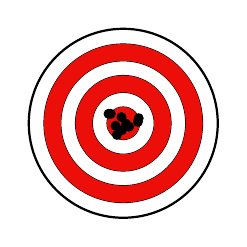
\begin{tikzpicture}[scale=0.4]
			\coordinate (O) at (0,0);
			\foreach \r in {0,...,5} \draw[thick] (O) circle (0.5cm + .5cm*\r);
			\draw[fill=red,draw=red] (O) circle (0.5);
			\draw[fill=red,draw=red,even odd rule] (O) circle (1.5cm) circle (1cm);
			\draw[fill=red,draw=red,even odd rule] (O) circle (2.5cm) circle (2cm);
			\draw plot [only marks, mark=*, mark size=4pt, domain=-2:1, samples=10] (rnd-0.5,rnd-0.5);
			\end{tikzpicture}
			                         &                              
			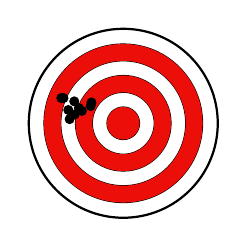
\begin{tikzpicture}[scale=0.4]
			\coordinate (O) at (0,0);
			\foreach \r in {0,...,5} \draw[thick] (O) circle (0.5cm + .5cm*\r);
			\draw[fill=red,draw=red] (O) circle (0.5);
			\draw[fill=red,draw=red,even odd rule] (O) circle (1.5cm) circle (1cm);
			\draw[fill=red,draw=red,even odd rule] (O) circle (2.5cm) circle (2cm);
			\draw plot [only marks, mark=*, mark size=4pt, domain=-2:1, samples=10] (rnd-2,rnd);
			\end{tikzpicture}
			\\
			Precise and Accurate     & Precise but Not Accurate     \\
			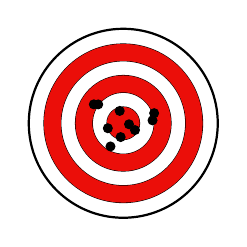
\begin{tikzpicture}[scale=0.4]
			\coordinate (O) at (0,0);
			\foreach \r in {0,...,5} \draw[thick] (O) circle (0.5cm + .5cm*\r);
			\draw[fill=red,draw=red] (O) circle (0.5);
			\draw[fill=red,draw=red,even odd rule] (O) circle (1.5cm) circle (1cm);
			\draw[fill=red,draw=red,even odd rule] (O) circle (2.5cm) circle (2cm);
			\draw plot [only marks, mark=*, mark size=4pt, domain=-2:1, samples=10] (rnd*2-1,rnd*2-1);
			\end{tikzpicture}
			                         &                              
			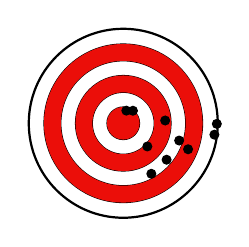
\begin{tikzpicture}[scale=0.4]
			\coordinate (O) at (0,0);
			\foreach \r in {0,...,5} \draw[thick] (O) circle (0.5cm + .5cm*\r);
			\draw[fill=red,draw=red] (O) circle (0.5);
			\draw[fill=red,draw=red,even odd rule] (O) circle (1.5cm) circle (1cm);
			\draw[fill=red,draw=red,even odd rule] (O) circle (2.5cm) circle (2cm);
			\draw plot [only marks, mark=*, mark size=4pt, domain=-2:1, samples=10] (rnd*3,rnd*3-2);
			\end{tikzpicture} \\
			Not Precise but Accurate & Not Precise and Not Accurate \\
		\end{tabular}
	\end{table}
\end{frame}

\begin{frame}{Ranking Estimators}
	We want our estimators to be both precise and accurate. There are two different ways to rank estimators
	\begin{enumerate}
		\item Minimum Variance Unbiased Estimator (MVUE)
		      \begin{itemize}
		      	\item Considering \alert{only} estimators that are unbiased, the best estimator is the one with the smallest variance
		      \end{itemize}
		\item Minimum Mean Squared Error (MMSE)
		      \begin{itemize}
		      	\item The estimator that has the smallest mean squared error
		      \end{itemize}
	\end{enumerate}
\end{frame}

\begin{frame}{Mean Squared Error}
	The Mean Squared Error essentially incorporates a trade off between bias and variance:
	\begin{center}
		MSE=Bias$^2$+Variance
	\end{center}
\end{frame}

\begin{frame}{Calculating Mean Squared Error}
	Recall our first estimator $\hat{\mu}_1:\frac{1}{4}X_1 + \frac{1}{4}X_2+\frac{1}{4}X_3$
	\vskip.8cm
	We calculated a bias of $-\frac{1}{4}\mu$
	\vskip.4cm
	We calculated a variance of $\frac{3}{16}\sigma^2$
	\vskip.8cm
	$$MSE(\hat{\mu}_1)=(-\frac{1}{4}\mu)^2+\frac{3}{16}\sigma^2=\frac{1}{16}\mu^2 + \frac{3}{16}\sigma^2$$
\end{frame}

\begin{frame}{Calculating Mean Squared Error}
	Recall our second estimator $\hat{\mu}_2: \frac{1}{2}\bar{X}_9+\frac{1}{2}\bar{X}_{12}$
	\vskip.8cm
	We calculated a bias of zero
	\vskip.4cm
	We calculated a variance of $\frac{7}{144}\sigma^2$
	\vskip.8cm
	$$MSE(\hat{\mu}_2)=0^2+\frac{7}{144}\sigma^2$$
\end{frame}

\begin{frame}{Comparing Estimators}
	Say $\mu=3$ and $\sigma^2=1$. Which estimator do we prefer under the MMSE?
	\vskip.4cm
	$$MSE(\hat{\mu}_1)=\frac{1}{16}\mu^2 + \frac{3}{16}\sigma^2=\frac{1}{16}\cdot 3^2+\frac{3}{16}\cdot1 = \frac{9}{16}+\frac{3}{16}=\frac{12}{16}=0.75$$
	\vskip.4cm
	$$MSE(\hat{\mu}_2)=\frac{7}{144}\sigma^2=\frac{7}{144}=0.049$$
	\vskip.4cm
	Since $MSE(\hat{\mu}_2)<MSE(\hat{\mu}_1)$, $\hat{\mu}_2$ is the preferred estimator
\end{frame}

\begin{frame}{Clicker Question}
	Which estimator, $\hat{\mu}_1$ or $\hat{\mu}_2$, is preferred under the Minimum Variance Unbiased Estimator?
	\vskip.6cm
	\begin{enumerate}[label=(\alph*)]
		\item $\hat{\mu}_1$
		\item $\hat{\mu}_2$
	\end{enumerate}
\end{frame}

\begin{frame}{Clicker Question -- Midterm Example}
	Given $X_1, X_2, ... , X_n$ are i.i.d. observations of random variable $X\sim N(\mu, \sigma^2)$. Answer the following question regarding these two estimators:
	$$\hat{\mu}_1=\frac{1}{3}X_1+\frac{1}{3}X_2$$
	$$\hat{\mu}_2=\frac{1}{4}X_1+\frac{3}{4}X_2$$
	\vskip.4cm
	What is the expectation of $\mu_1$?
	\begin{enumerate}[label=(\alph*)]
		\item $\mu$
		\item $\frac{2}{3}\mu$ %
		\item $\-\frac{1}{3}\mu$
		\item $0$
	\end{enumerate}
\end{frame}

\begin{frame}{Clicker Question -- Midterm Example}
	Given $X_1, X_2, ... , X_n$ are i.i.d. observations of random variable $X\sim N(\mu, \sigma^2)$. Answer the following question regarding these two estimators:
	$$\hat{\mu}_1=\frac{1}{3}X_1+\frac{1}{3}X_2$$
	$$\hat{\mu}_2=\frac{1}{4}X_1+\frac{3}{4}X_2$$
	\vskip.4cm
	What is the expectation of $\mu_2$?
	\begin{enumerate}[label=(\alph*)]
		\item $\mu$ %
		\item $\frac{2}{3}\mu$
		\item $-\frac{1}{3}\mu$
		\item $0$
	\end{enumerate}
\end{frame}

\begin{frame}{Clicker Question -- Midterm Example}
	Given $X_1, X_2, ... , X_n$ are i.i.d. observations of random variable $X\sim N(\mu, \sigma^2).$ Answer the following question regarding these two estimators:
	$$\hat{\mu}_1=\frac{1}{3}X_1+\frac{1}{3}X_2$$
	$$\hat{\mu}_2=\frac{1}{4}X_1+\frac{3}{4}X_2$$
	
	\vskip.4cm
	What is the variance of $\mu_1$?
	\begin{enumerate}[label=(\alph*)]
		\item $\frac{2}{3}\sigma^2$ 
		\item $\frac{2}{9}\sigma^2$
		\item $\sigma^2$
		\item None of the above
	\end{enumerate}
\end{frame}

\begin{frame}{Clicker Question -- Midterm Example}
	Given $X_1, X_2, ... , X_n$ are i.i.d. observations of random variable $X\sim N(\mu, \sigma^2)$. Answer the following question regarding these two estimators:
	$$\hat{\mu}_1=\frac{1}{3}X_1+\frac{1}{3}X_2$$
	$$\hat{\mu}_2=\frac{1}{4}X_1+\frac{3}{4}X_2$$
	\vskip.4cm
	What is the variance of $\mu_2$?
	\begin{enumerate}[label=(\alph*)]
		\item $\frac{10}{16}\sigma^2$
		\item $\sigma^2$
		\item $\frac{10}{4}\sigma^2$
		\item None of the above
	\end{enumerate}
\end{frame}

\begin{frame}{Clicker Question -- Midterm Example}
	Suppose $\mu=1$ and $\sigma^2=1$, find the MSE for each and determine which estimator is preferred under MMSE? Which is preferred under MVUE? 
	\begin{enumerate}[label=(\alph*)]
		\item $\hat{\mu}_1$ is preferred under both
		\item $\hat{\mu}_2$ is preferred under both
		\item $\hat{\mu}_1$ is preferred under MMSE; $\hat{\mu}_2$ is preferred under MVUE %
		\item $\hat{\mu}_1$ is preferred under MVUE; $\hat{\mu}_2$ is preferred under MMSE
	\end{enumerate}
\end{frame}

\end{document}